\chapter{Validação da Aceitação Tecnológica}
\label{cap:validacao-tam}

Este capítulo apresenta os resultados da avaliação de aceitação tecnológica dos dashboards públicos desenvolvidos nesta pesquisa, conduzida com o instrumento TAM descrito na Seção~\ref{sec:instrumento-tam}. A avaliação cumpre a etapa de validação do artefato prevista no ciclo da Design Science: após a construção do sistema (Capítulo~\ref{cap:implementacao}) e sua aplicação ao estudo de caso (Capítulo~\ref{cap:resultados}), o artefato foi submetido ao julgamento de potenciais usuários reais, que exploraram os dashboards hospedados publicamente e registraram suas percepções de utilidade, facilidade de uso e intenção de uso, além de avaliações complementares sobre a interface e os diagnósticos gerados pela IA.

\section{Perfil dos Participantes}
\label{sec:perfil-participantes}

Participaram da avaliação cinco respondentes ($n=5$), recrutados por conveniência entre os perfis-alvo da ferramenta: profissionais da gestão pública municipal e membros da comunidade acadêmica de instituições de ensino superior da região. A Tabela~\ref{tab:perfil-tam} resume o perfil dos participantes, identificados de A1 a A5 para preservar o anonimato.

\begin{table}[h!]
    \centering
    \caption{Perfil dos participantes da avaliação TAM}
    \label{tab:perfil-tam}
    \begin{tabular}{clc}
        \hline
        \textbf{ID} & \textbf{Vínculo institucional} & \textbf{Data da avaliação} \\
        \hline
        A1 & Instituto de previdência municipal (Mossoró-RN) & 25/02/2026 \\
        A2 & Instituto de previdência municipal (Mossoró-RN) & 25/02/2026 \\
        A3 & Universidade do Estado do Rio Grande do Norte (UERN) & 30/03/2026 \\
        A4 & UFERSA -- Docente de Engenharia de Produção & 30/03/2026 \\
        A5 & Setor administrativo-financeiro & 30/03/2026 \\
        \hline
    \end{tabular}
    \legend{Fonte: Elaborado pelo autor (2026).}
\end{table}

A composição da amostra combina os dois perfis de usuário previstos para a ferramenta: A1, A2 e A5 representam a perspectiva da gestão pública e administrativa, principal público-alvo dos diagnósticos municipais, enquanto A3 e A4 representam a perspectiva acadêmica, com olhar metodológico sobre a apresentação e a consistência dos dados. Todos os participantes exploraram os dashboards públicos hospedados em \url{https://dashboard-ods-mossoro.netlify.app/} antes de responder ao questionário.

\section{Resultados Quantitativos por Construto}
\label{sec:resultados-tam}

A Tabela~\ref{tab:respostas-tam} apresenta as respostas individuais dos cinco participantes aos oito itens do instrumento, na escala Likert de 1 a 5, juntamente com a média de cada item.

\begin{table}[h!]
    \centering
    \caption{Respostas individuais aos itens TAM (escala Likert 1--5)}
    \label{tab:respostas-tam}
    \begin{tabular}{clcccccc}
        \hline
        \textbf{Item} & \textbf{Construto} & \textbf{A1} & \textbf{A2} & \textbf{A3} & \textbf{A4} & \textbf{A5} & \textbf{Média} \\
        \hline
        PU1  & Utilidade  & 5 & 4 & 4 & 3 & 4 & 4,0 \\
        PU2  & Utilidade  & 5 & 4 & 4 & 4 & 4 & 4,2 \\
        PU3  & Utilidade  & 5 & 4 & 5 & 3 & 4 & 4,2 \\
        PFU1 & Facilidade & 5 & 4 & 2 & 4 & 4 & 3,8 \\
        PFU2 & Facilidade & 5 & 4 & 2 & 4 & 4 & 3,8 \\
        PFU3 & Facilidade & 5 & 4 & 4 & 4 & 4 & 4,2 \\
        ICU1 & Intenção   & 5 & 3 & 4 & 3 & 4 & 3,8 \\
        ICU2 & Intenção   & 5 & 4 & 4 & 3 & 4 & 4,0 \\
        \hline
        \multicolumn{2}{l}{\textbf{Média por respondente}} & \textbf{5,00} & \textbf{3,88} & \textbf{3,63} & \textbf{3,50} & \textbf{4,00} & \textbf{4,00} \\
        \hline
    \end{tabular}
    \legend{Fonte: Elaborado pelo autor (2026).}
\end{table}

A partir das respostas individuais, foram calculadas as médias por construto, apresentadas na Tabela~\ref{tab:medias-construtos} e na Figura~\ref{fig:tam-medias}.

\begin{table}[h!]
    \centering
    \caption{Médias por construto do TAM}
    \label{tab:medias-construtos}
    \begin{tabular}{lccc}
        \hline
        \textbf{Construto} & \textbf{Itens} & \textbf{Média} & \textbf{Amplitude observada} \\
        \hline
        Percepção de Utilidade (PU) & PU1--PU3 & 4,13 & 3--5 \\
        Percepção de Facilidade de Uso (PFU) & PFU1--PFU3 & 3,93 & 2--5 \\
        Intenção Comportamental de Uso (ICU) & ICU1--ICU2 & 3,90 & 3--5 \\
        \hline
        \textbf{Geral (8 itens)} & -- & \textbf{4,00} & 2--5 \\
        \hline
    \end{tabular}
    \legend{Fonte: Elaborado pelo autor (2026).}
\end{table}

\begin{figure}[h!]
    \centering
    \caption{Médias dos itens TAM por construto}
    \label{fig:tam-medias}
    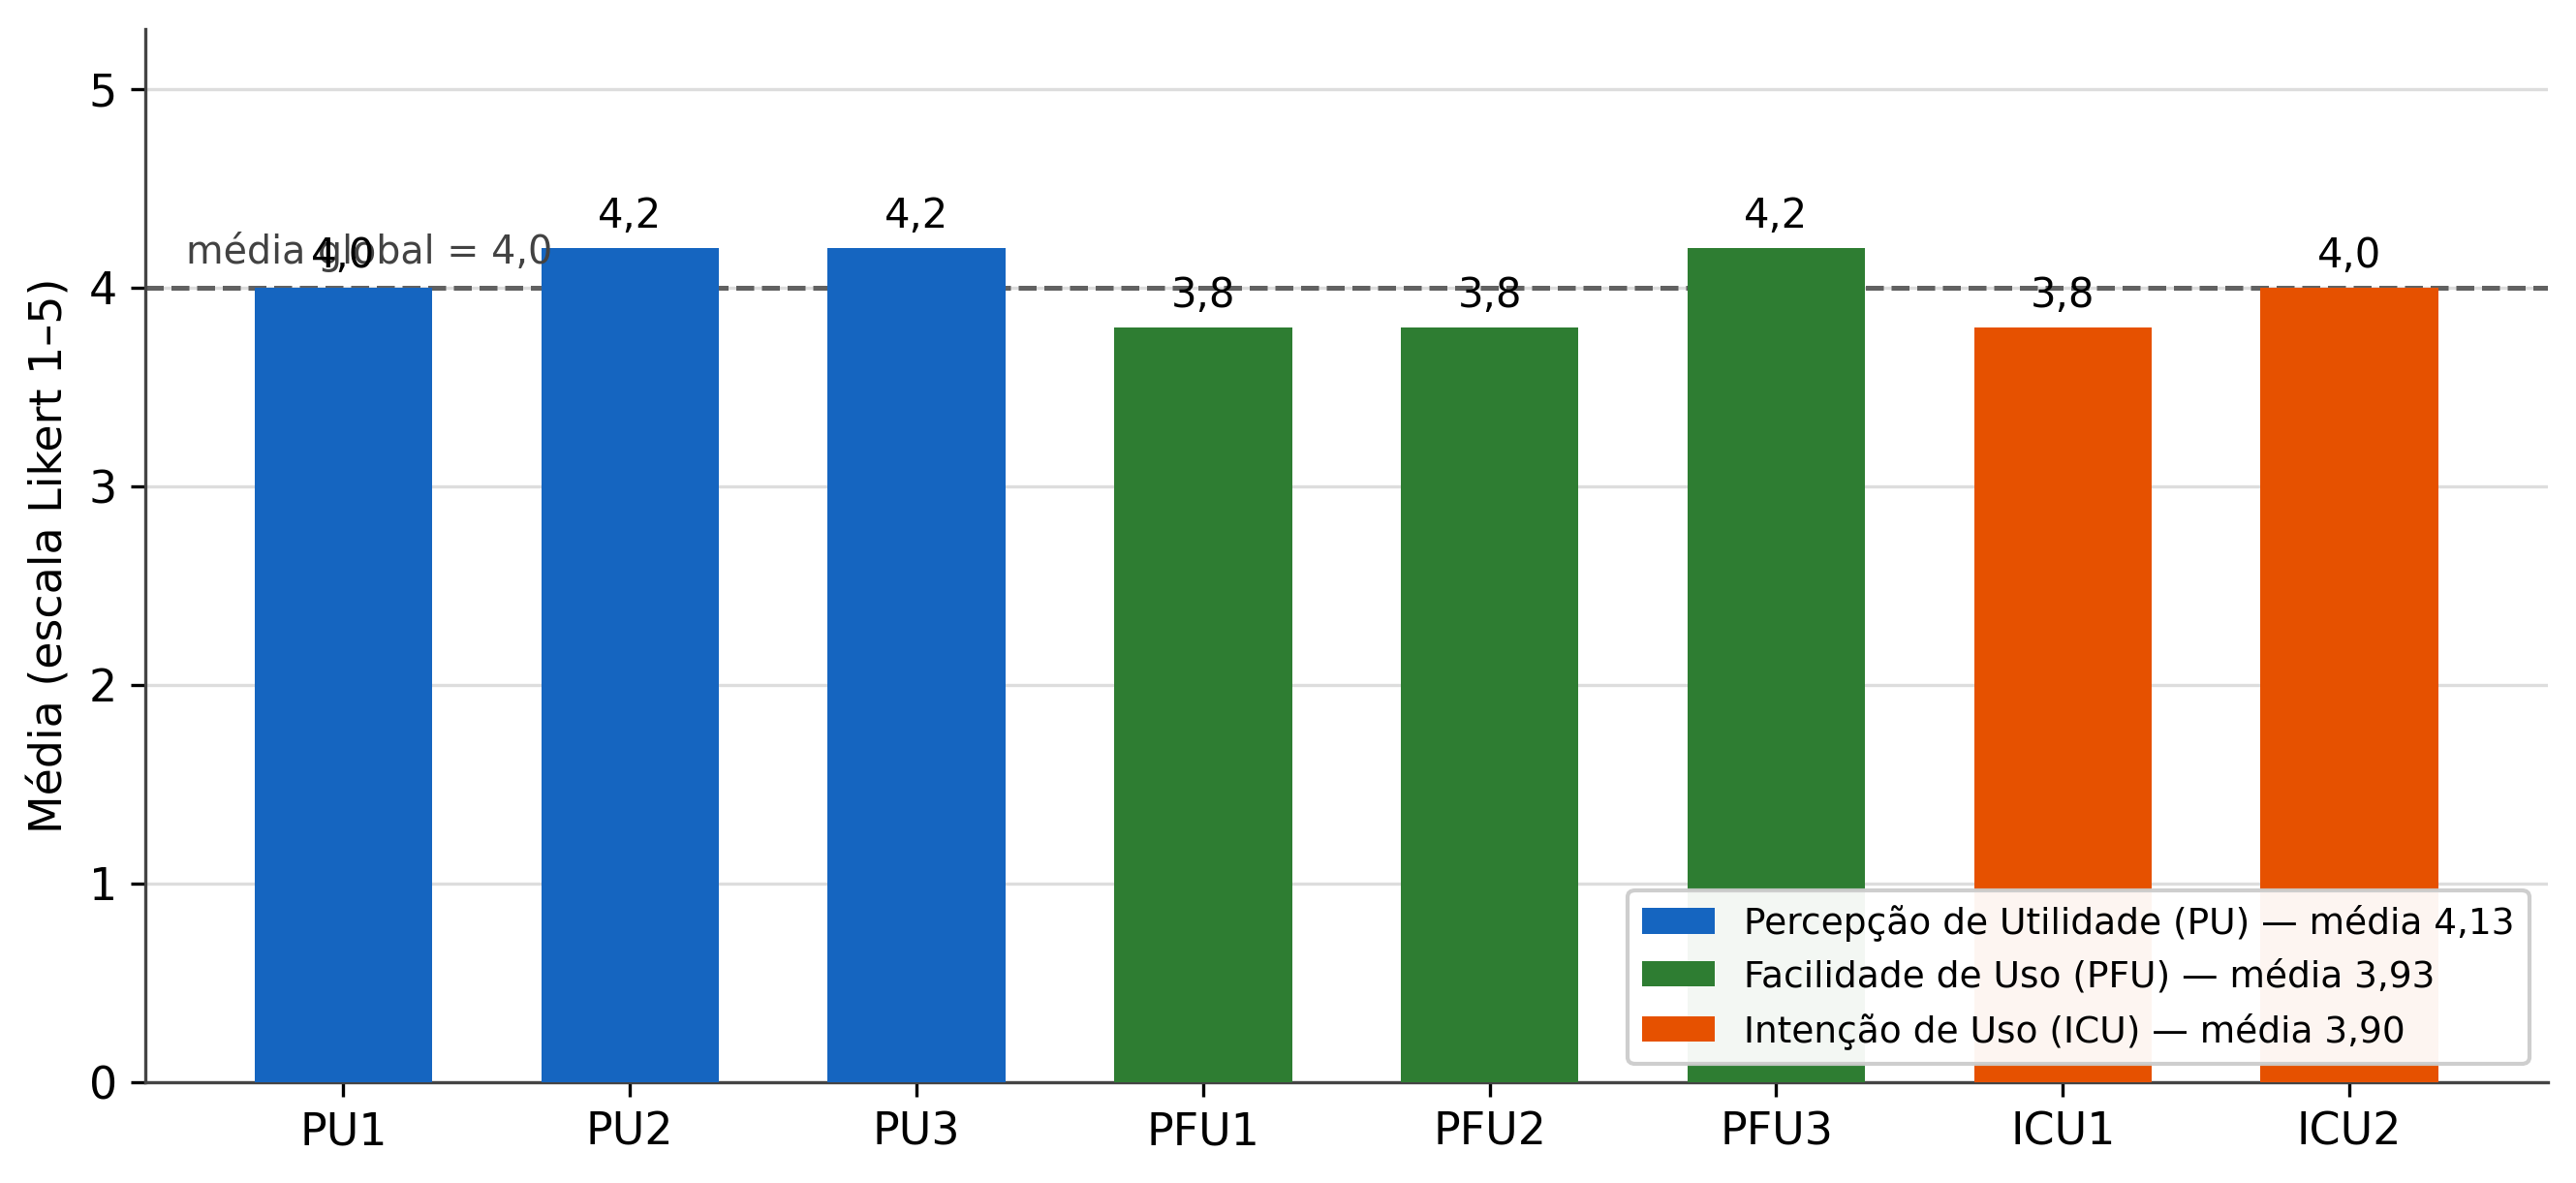
\includegraphics[width=0.95\textwidth]{figuras/tam-medias-construtos}
    \legend{Fonte: Elaborado pelo autor (2026).}
\end{figure}

Os três construtos apresentaram médias iguais ou superiores a 3,9 em escala de 5 pontos, com média global de 4,00 -- valor correspondente ao nível ``Concordo'' da escala. A Percepção de Utilidade obteve a maior média (4,13), com nenhuma resposta abaixo do ponto neutro: os cinco avaliadores concordaram, em diferentes graus, que os dashboards melhoram o desempenho na tomada de decisão e fornecem informações relevantes às suas responsabilidades. Esse resultado é particularmente significativo por vir, em sua maioria, de profissionais da gestão pública, público a quem o artefato se destina.

A Percepção de Facilidade de Uso apresentou média ligeiramente inferior (3,93) e a maior dispersão entre os construtos (amplitude de 2 a 5). Essa dispersão decorre integralmente do avaliador A3, que atribuiu nota 2 (``Discordo'') aos itens PFU1 (facilidade de aprendizado) e PFU2 (clareza da interação), embora tenha avaliado positivamente a navegação (PFU3 = 4) e atribuído notas máximas à satisfação com os dados e diagnósticos. Esse padrão sugere que a dificuldade relatada concentra-se na curva de aprendizado inicial da ferramenta, e não no acesso à informação em si -- interpretação corroborada pelo fato de A3 ter avaliado todos os aspectos técnicos da interface como ``Bom'' e manifestado intenção de uso positiva (ICU = 4).

A Intenção Comportamental de Uso (3,90) manteve-se próxima das demais, com as únicas respostas neutras vindas de A2 e A4 no item ICU1, relativo ao uso regular para acompanhamento de indicadores da própria área. Esse resultado é coerente com o perfil dos respondentes: para avaliadores cuja rotina não envolve diretamente o monitoramento de ODS, a intenção de uso regular tende a ser naturalmente mais moderada do que a percepção de utilidade da ferramenta em abstrato.

\section{Avaliação Complementar dos Dashboards}
\label{sec:avaliacao-complementar}

Nas questões complementares de satisfação, os dashboards obtiveram resultados consistentemente positivos. Na escala de 1 a 5, a satisfação com a clareza e precisão dos dados dos dashboards principais alcançou média 4,6 (três notas 5 e duas notas 4), mesmo valor obtido pela satisfação com a clareza e profundidade da tela de diagnósticos (4,6). Nenhum participante atribuiu nota inferior a 4 em qualquer das duas escalas.

Quanto à preferência entre os painéis, quatro dos cinco avaliadores consideraram que ambos os dashboards são igualmente úteis às suas atividades, e um (A4) indicou preferência pelo dashboard específico, com foco em detalhamento e diagnóstico. Nenhum respondente selecionou a opção ``Nenhum é útil''. A Tabela~\ref{tab:aspectos-interface} consolida a avaliação dos quatro aspectos técnicos da interface.

\begin{table}[h!]
    \centering
    \caption{Avaliação dos aspectos técnicos da interface ($n=5$)}
    \label{tab:aspectos-interface}
    \begin{tabular}{lcccc}
        \hline
        \textbf{Aspecto} & \textbf{Ruim} & \textbf{Regular} & \textbf{Bom} & \textbf{Excelente} \\
        \hline
        Velocidade de carregamento & 0 & 0 & 3 & 2 \\
        Design e estética visual & 0 & 0 & 4 & 1 \\
        Organização e fluxo de navegação & 0 & 0 & 3 & 2 \\
        Capacidade de filtrar e detalhar dados (\textit{drill-down}) & 0 & 1 & 3 & 1 \\
        \hline
    \end{tabular}
    \legend{Fonte: Elaborado pelo autor (2026).}
\end{table}

Todos os aspectos concentraram-se nos níveis ``Bom'' e ``Excelente'', com uma única avaliação ``Regular'', atribuída por A4 à capacidade de filtrar e detalhar dados. Essa avaliação é consistente com a sugestão de melhoria registrada pela mesma participante na questão aberta, discutida na Seção~\ref{sec:analise-qualitativa}, e indica que a filtragem avançada é o ponto da interface com maior espaço de evolução.

Na questão sobre a utilidade dos diagnósticos gerados pela IA, as opções mais selecionadas foram ``Ajudam a identificar áreas críticas para intervenção'' (três respondentes) e ``Oferecem uma visão clara do progresso de Mossoró nos ODS'' (três respondentes). Um respondente (A2) considerou os diagnósticos ``fundamentais para o planejamento estratégico'' de sua área, e um (A4) marcou a opção crítica ``São muito superficiais e pouco acionáveis''. Nenhum participante declarou não utilizar os diagnósticos. No ranqueamento de importância entre as informações dos dashboards principais e os diagnósticos gerados pela IA, três avaliadores atribuíram importância máxima a ambos os componentes; A4 priorizou os dashboards principais em detrimento dos diagnósticos, e A5 fez o movimento inverso, priorizando os diagnósticos da IA. Em conjunto, os dois componentes foram considerados ``mais importantes'' por quatro dos cinco avaliadores cada, indicando que a combinação entre exploração quantitativa e síntese qualitativa automatizada -- e não apenas um dos elementos -- é percebida como o valor central da ferramenta.

\section{Análise Qualitativa das Respostas Abertas}
\label{sec:analise-qualitativa}

As três perguntas abertas receberam quatro contribuições textuais, transcritas integralmente no Quadro~\ref{tab:respostas-abertas}.

\begin{table}[h!]
    \centering
    \caption{Respostas às perguntas abertas do questionário}
    \label{tab:respostas-abertas}
    \begin{tabular}{clp{8.5cm}}
        \hline
        \textbf{ID} & \textbf{Pergunta} & \textbf{Resposta} \\
        \hline
        A1 & Indicadores faltantes & ``Propostas do que fazer para melhorar tal serviço, etc.'' \\
        A4 & Indicadores faltantes & ``Poderia ter um filtro no dashboard (`análise detalhada'), similar ao do excel.'' \\
        A1 & Dificuldades encontradas & ``Nenhum problema encontrado.'' \\
        A1 & Comentários finais & ``Excelente iniciativa.'' \\
        \hline
    \end{tabular}
    \legend{Fonte: Elaborado pelo autor (2026).}
\end{table}

Da análise das respostas emergem três achados qualitativos:

\begin{enumerate}
    \item \textbf{Demanda por recomendações acionáveis}: a sugestão de A1 -- incluir ``propostas do que fazer para melhorar tal serviço'' -- converge com a crítica de A4 sobre a superficialidade dos diagnósticos e aponta para a mesma necessidade: aproximar o diagnóstico da prescrição. Embora os diagnósticos gerados pela IA já incluam recomendações estratégicas (Seção~\ref{sec:diagnosticos-automaticos}), o achado indica que essas recomendações precisam ganhar mais destaque na interface, idealmente vinculadas a cada estabelecimento ou dimensão específica, e não apenas ao diagnóstico geral.
    \item \textbf{Demanda por filtragem avançada}: a sugestão de A4, docente de Engenharia de Produção familiarizada com ferramentas de análise de dados, propõe filtros de tabela semelhantes aos do Microsoft Excel na tela de análise detalhada. A sugestão é tecnicamente viável -- os dashboards já carregam os registros individuais em memória -- e foi incorporada à lista de melhorias futuras da ferramenta, em conjunto com a única avaliação ``Regular'' atribuída ao \textit{drill-down} pela mesma avaliadora.
    \item \textbf{Ausência de problemas técnicos}: nenhum participante relatou dados incorretos, \textit{links} quebrados, lentidão ou confusão de navegação. O único registro na pergunta sobre dificuldades foi explicitamente positivo (``Nenhum problema encontrado''), o que corrobora as avaliações de velocidade de carregamento e organização da interface da Tabela~\ref{tab:aspectos-interface} e sugere que a estratégia de páginas estáticas hospedadas em CDN (Seção~\ref{sec:dashboards-publicos}) atende aos requisitos de desempenho percebido.
\end{enumerate}

O comentário final de A1 (``Excelente iniciativa''), somado às médias elevadas de satisfação, completa um quadro qualitativo favorável: a ferramenta é percebida como útil e funcional, e as críticas registradas são construtivas e específicas, direcionadas a evoluções incrementais da interface e não a problemas estruturais da abordagem.

\section{Ameaças à Validade da Avaliação}
\label{sec:ameacas-validade-tam}

Os resultados desta avaliação devem ser interpretados à luz de limitações metodológicas importantes, que delimitam o alcance das conclusões.

\textbf{Tamanho da amostra ($n=5$)}: a limitação mais relevante é o número reduzido de respondentes. Com cinco participantes, os resultados não permitem inferência estatística sobre a população de potenciais usuários: as médias reportadas são estatísticas descritivas da amostra, e variações de um único respondente alteram sensivelmente os valores agregados -- como ilustra o efeito das notas de A3 sobre a média do construto PFU. Pela mesma razão, não foram calculados coeficientes de consistência interna (como o alfa de Cronbach) nem testes de significância, cuja aplicação seria estatisticamente inadequada nesse tamanho amostral. A avaliação deve, portanto, ser lida como um estudo exploratório de aceitação, e não como uma validação psicométrica do instrumento ou uma medição populacional.

\textbf{Amostragem por conveniência e autosseleção}: os participantes foram recrutados na rede de contatos profissional e acadêmica do pesquisador, o que introduz risco de viés de cortesia (tendência a avaliações benevolentes) e de autosseleção (responderam aqueles com maior disposição favorável à iniciativa). A coleta anônima via formulário eletrônico mitiga parcialmente esse risco, mas não o elimina. A presença de críticas específicas nas respostas -- as notas 2 de A3 em facilidade de uso, a avaliação ``Regular'' e a marcação de ``superficiais e pouco acionáveis'' por A4 -- sugere, contudo, que os respondentes se sentiram à vontade para registrar discordâncias, o que aumenta a credibilidade das avaliações positivas.

\textbf{Exposição única e de curta duração}: os participantes exploraram os dashboards em uma única sessão, antes de responder ao questionário. A intenção de uso declarada (ICU) em exposição única não equivale ao uso continuado real, que o TAM se propõe a prever; estudos longitudinais seriam necessários para verificar se a intenção se converte em adoção efetiva \cite{venkatesh2000}.

\textbf{Escopo do artefato avaliado}: a avaliação cobriu os dashboards públicos e as telas de diagnóstico -- a camada de apresentação do sistema --, mas não os componentes internos do pipeline (coleta, filtragem, análise por aspecto), cuja validação seguiu estratégias distintas, descritas nos Capítulos~\ref{cap:implementacao} e~\ref{cap:resultados}.

Apesar dessas limitações, a avaliação cumpre seu papel no ciclo da Design Science: fornece evidência inicial de que o artefato é percebido como útil e utilizável pelos perfis de usuário a que se destina, identifica pontos concretos de melhoria (recomendações mais acionáveis e filtragem avançada) e estabelece um protocolo de avaliação replicável -- instrumento, procedimento e métricas -- que pode ser reaplicado com amostras maiores e mais diversas em trabalhos futuros.

\section{Síntese do Capítulo}
\label{sec:sintese-validacao}

A avaliação de aceitação tecnológica com cinco potenciais usuários -- três da gestão pública e administrativa e dois da academia -- indicou percepção favorável dos dashboards nos três construtos do TAM: utilidade percebida de 4,13, facilidade de uso de 3,93 e intenção de uso de 3,90, em escala de 5 pontos, com média global de 4,00. As escalas complementares de satisfação alcançaram 4,6 tanto para os dados dos dashboards principais quanto para a tela de diagnósticos, e nenhum problema técnico foi relatado. A análise qualitativa identificou duas demandas convergentes de evolução -- recomendações mais acionáveis e filtros avançados na análise detalhada -- que constituem o roteiro natural de melhoria da camada de visualização. Dados o tamanho e a natureza da amostra, esses resultados configuram evidência exploratória, e não conclusiva, de aceitação do artefato.
